\documentclass[aspectratio=169]{beamer}
\usetheme{Madrid}
\usecolortheme{beaver}
\usepackage[utf8]{inputenc}
\usepackage[T1]{fontenc}
\usepackage{tikz}
\usepackage{amssymb}
\usepackage{graphicx}
\setbeamertemplate{navigation symbols}{}
\setbeamercolor{title}{fg=white,bg=cyan!60!black}
\setbeamercolor{frametitle}{fg=white,bg=cyan!50!black}
\setbeamercolor{block title}{bg=cyan!15,fg=black}
\setbeamercolor{block body}{bg=cyan!5,fg=black}

\title{Story Studio 3 — Make It Click}
\subtitle{onclick — a button that actually does something when pressed}
\author{ByteForge --- Grade 7 --- Game Maker --- Week Overview}
\date{}

\begin{document}

\begin{frame}
    \titlepage
\end{frame}

\begin{frame}{This Week's Plan}
    \begin{itemize}
        \item Lesson 1: Click to Reveal
        \item Lesson 2: Click for More
        \item Lesson 3: Both at Once
        \item Lesson 4: Button Talks Back
        \item[$\bigstar$] BOSS --- The Big Reveal (\texttt{lessonBoss.tex})
    \end{itemize}
\end{frame}

\begin{frame}{Real-World Example}
    \Large
    Click an "Add to cart" button on a real shopping site — the label changing to "Added \textbackslash\{\}checkmark" or a counter updating is exactly this week's "button talks back" idea, live in production software. A Minecraft crafting-table "craft" button is the same: click it, and it visibly does something (moves items) right there.
\end{frame}


\begin{frame}{Image}
    \begin{center}
    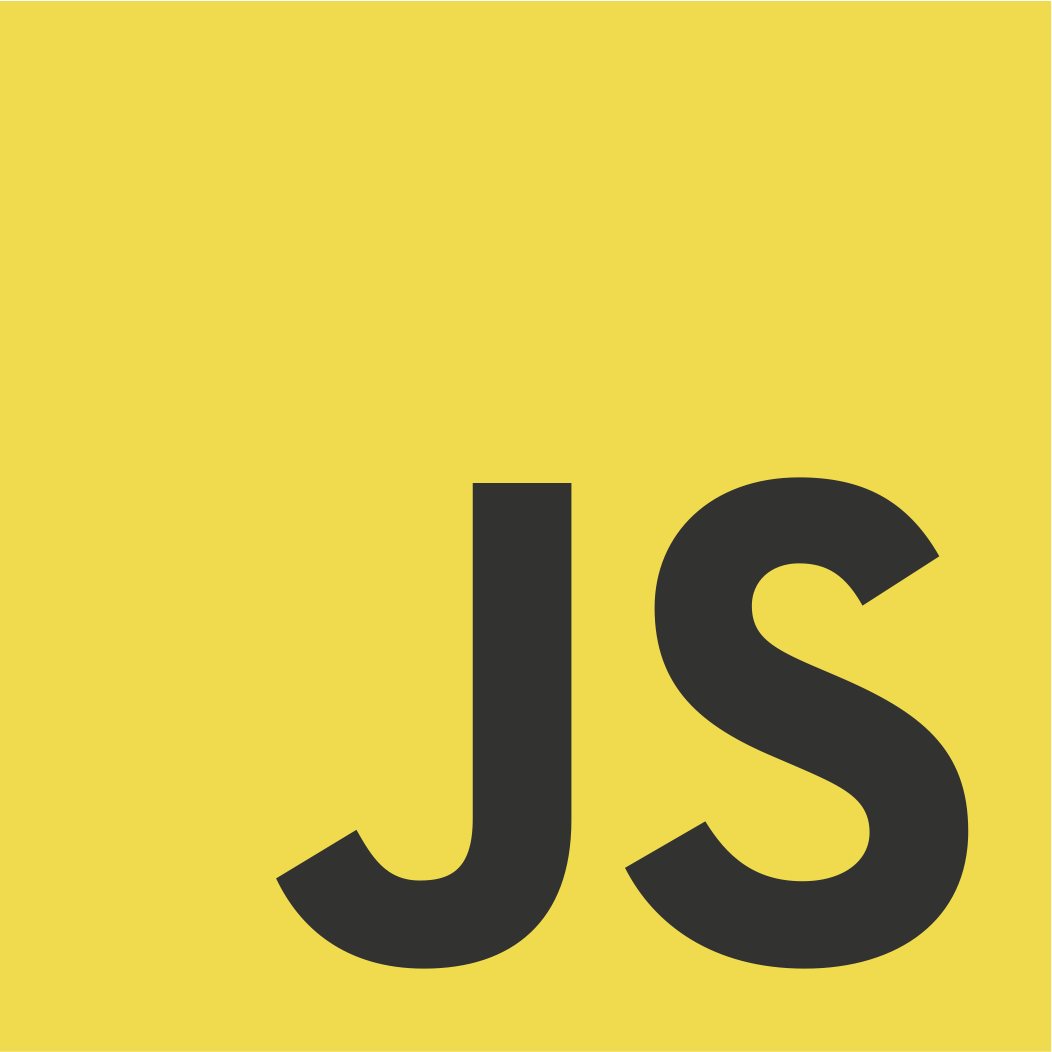
\includegraphics[width=0.55\textwidth]{../images/js.png}

    \small JavaScript logo — Chris Williams, public domain, via Wikimedia Commons
    \end{center}
\end{frame}

\begin{frame}{Let Them Discover}
    \Large
    Find a button on any app or website that changes itself when clicked (a like button, a "show password" eye icon, a checkbox). What exactly changes — text, colour, icon? Nothing else on the page needs to change too.
\end{frame}

\begin{frame}{Files in This Folder}
    \small
    \begin{itemize}
        \item \texttt{lesson1.tex} --- Click to Reveal
        \item \texttt{lesson2.tex} --- Click for More
        \item \texttt{lesson3.tex} --- Both at Once
        \item \texttt{lesson4.tex} --- Button Talks Back
        \item \texttt{lessonBoss.tex} --- BOSS: The Big Reveal
    \end{itemize}
    \vspace{0.5em}
    \normalsize Each lesson file is its own short deck --- open the one for
    the specific day you're teaching, not this whole overview.
\end{frame}

\end{document}
